% PURGE: Projected Unlearning via Retain-Guided Erasure
% AAAI 2026 Submission (Anonymous)

\def\aaaianonymous{true}

\documentclass[letterpaper]{article} % DO NOT CHANGE THIS
\usepackage[submission]{aaai2026} % Anonymous submission
\usepackage{times} % DO NOT CHANGE THIS
\usepackage{helvet} % DO NOT CHANGE THIS
\usepackage{courier} % DO NOT CHANGE THIS
\usepackage[hyphens]{url} % DO NOT CHANGE THIS
\usepackage{graphicx} % DO NOT CHANGE THIS
\urlstyle{rm} % DO NOT CHANGE THIS
\def\UrlFont{\rm} % DO NOT CHANGE THIS
\usepackage{natbib} % DO NOT CHANGE THIS AND DO NOT ADD ANY OPTIONS TO IT
\usepackage{caption} % DO NOT CHANGE THIS AND DO NOT ADD ANY OPTIONS TO IT
\frenchspacing % DO NOT CHANGE THIS
\setlength{\pdfpagewidth}{8.5in} % DO NOT CHANGE THIS
\setlength{\pdfpageheight}{11in} % DO NOT CHANGE THIS

% Allowed additional packages
\usepackage{amsmath,amssymb}
\usepackage{booktabs}
\usepackage{algorithm}
\usepackage{algorithmic}
\usepackage{xcolor}
\usepackage{pifont}
\usepackage{multirow}
\usepackage{subcaption}

\graphicspath{{../images/}}

\setcounter{secnumdepth}{2}

\pdfinfo{
/TemplateVersion (2026.1)
}

% --- Macros ---
\newcommand{\ours}{\textsc{Purge}}
\newcommand{\klr}{\texttt{kl\_retain}}
\newcommand{\KL}{\mathrm{KL}}
\newcommand{\CE}{\mathrm{CE}}
\newcommand{\Df}{\mathcal{D}_f}
\newcommand{\Dr}{\mathcal{D}_r}
\newcommand{\gf}{g_{\mathrm{f}}}
\newcommand{\gr}{g_{\mathrm{r}}}
\newcommand{\gproj}{\tilde{g}_{\mathrm{f}}}
\newcommand{\lossf}{\mathcal{L}_{\mathrm{f}}}
\newcommand{\lossr}{\mathcal{L}_{\mathrm{r}}}
\newcommand{\lossrep}{\mathcal{L}_{\mathrm{rep}}}
\newcommand{\losskd}{\mathcal{L}_{\mathrm{KD}}}
\newcommand{\cmark}{{\color{green!60!black}\ding{51}}}
\newcommand{\xmark}{{\color{red!70!black}\ding{55}}}
\newcommand{\pmark}{{\color{orange!80!black}$\sim$}}

\newtheorem{theorem}{Theorem}

% ============================================================
\title{PURGE: Projected Unlearning via Retain-Guided Erasure}

\author{
    Anonymous Authors
}
\affiliations{
    Anonymous Affiliations
}

% ============================================================
\begin{document}
\maketitle

% ============================================================
\begin{abstract}
Machine unlearning must remove the influence of specific training data while preserving model utility---a forget--retain trade-off dual to the stability--plasticity trade-off of continual learning.
We exploit this duality and adapt A-GEM gradient projection so that every projected update provably does not increase the mini-batch retain loss beyond an $O(\eta^2)$ smoothness term, giving the first \emph{exact per-step retain-safety guarantee}---for the (momentum-free) optimiser actually used---in approximate machine unlearning.
We instantiate this idea in \ours{} (\textbf{P}rojected \textbf{U}nlearning via \textbf{R}etain-\textbf{G}uided \textbf{E}rasure), which combines (i)~the projected gradient update, (ii)~a retain-confusion forget objective that targets the model's natural output distribution on retained data, and (iii)~dual stopping with explicit retain-loss and forget-accuracy budgets.
The guarantee is formalised as Theorem~\ref{thm:retain_safety}; a separation theorem (Theorem~\ref{thm:separation}) then shows that no prior method---GA, SCRUB, or SalUn---carries this per-step guarantee.
Across six datasets and 31 class-level forgetting tasks with ResNet-18 (three seeds each on the five 10-class datasets), \ours{} achieves per-dataset mean forget accuracy $\le 6.3$\% (excl.\ STL-10), retain accuracy $> 95$\% ($91$\% on CIFAR-100), and MIA AUROC $\approx 0.5$.
Replacing BatchNorm with GroupNorm eliminates a BN-recalibration vulnerability ($\Delta F = 0$) while keeping forget, retain, and test accuracy competitive on CIFAR-10 (Table~\ref{tab:comparison}).
\end{abstract}

% ============================================================
\section{Introduction}\label{sec:intro}

Trained models increasingly need to demonstrably \emph{forget} specific data---whether to honour data-deletion requests, revoke expired licences, or remove poisoned samples.
Retraining from scratch satisfies this exactly but is computationally prohibitive: a ResNet-18 on CIFAR-10 takes ${\sim}45$ minutes on a single A100; on production-scale models, days to weeks.
The machine unlearning question is: \emph{can we modify a trained model so that it behaves as if a specified subset were absent from training, without the cost of full retraining?}

Existing approximate unlearning methods each occupy a different point on the privacy--utility frontier, and each has a critical gap.
Gradient ascent (GA) \citep{thudi2022unrolling} maximises forget-set loss but has no mechanism to protect retain-set accuracy, collapsing test accuracy to ${\sim}38$\% on CIFAR-10.
SalUn \citep{fan2024salun} selectively masks salient weights and applies random-label updates---effective in practice, but with no formal retain-performance guarantee and no control over how much is forgotten: its random-label masking drives forget accuracy to $0$\% with no tunable target.
SCRUB \citep{kurmanji2023unbounded} alternates forget and retain steps balanced by a weight $\lambda$, but the result is brittle: mistune $\lambda$ and either forgetting stalls (FA~$= 52.6$\%) or retain accuracy collapses (RA~$= 93.7$\%).
Critically, \textbf{none of these methods provides a per-step guarantee that retain-set performance is preserved.}

\begin{figure}[t]
\centering
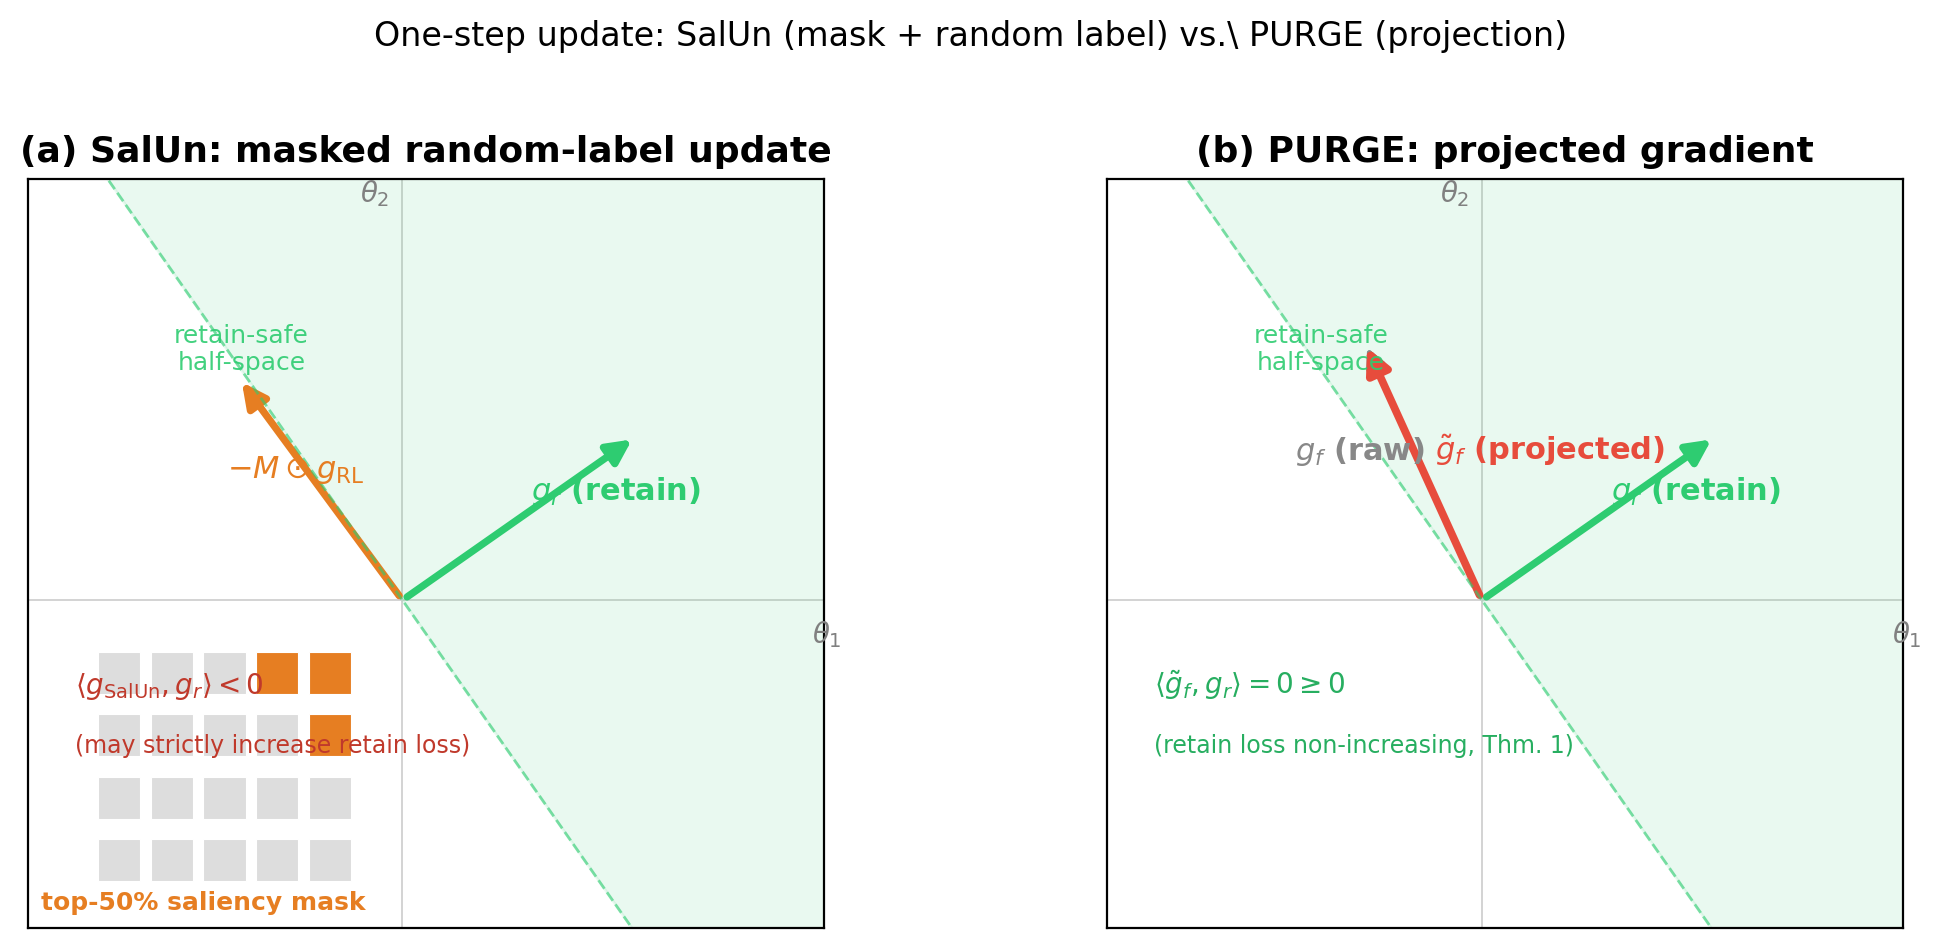
\includegraphics[width=\columnwidth]{fig_purge_vs_salun.png}
\caption{\textbf{One-step geometry: SalUn vs.\ \ours{}.} \textbf{Left:} SalUn's masked random-label gradient has no constraint on its inner product with the retain gradient $\gr$---a single step can land outside the retain-safe half-space. \textbf{Right:} \ours{} projects the forget gradient $\gf$ so that $\langle \gproj, \gr \rangle \ge 0$ at every step, so the clipped update does not increase the sampled retain loss beyond an $O(\eta^2)$ term (Theorem~\ref{thm:retain_safety}).}
\label{fig:geometry}
\end{figure}

\paragraph{Our insight.}
Continual learning (CL) protects old-task knowledge while learning new tasks; machine unlearning (MU) protects retained knowledge while erasing specific data---the same trade-off in opposite directions.
This duality has been noted conceptually \citep{kurmanji2023unbounded,nguyen2020variational} and, more recently, used as a \emph{soft} gradient regulariser \citep{patel2025learning}---but never as a hard, per-step update rule with a formal guarantee.
We do exactly that: we adapt A-GEM gradient projection \citep{chaudhry2019agem}---the workhorse of episodic-memory CL---as the \emph{primary update operator} for unlearning.
The forget gradient is projected onto the retain-safe half-space $\{g : \langle g, \gr\rangle \ge 0\}$ \emph{before every parameter update} (Figure~\ref{fig:geometry}).
This single mechanism yields the per-step retain-safety guarantee; the remaining components of \ours{} build on it.

\paragraph{Contributions.}
We make three contributions, each addressing a specific challenge in approximate unlearning.

\textbf{(1) Constrained optimisation framing.}
Prior methods frame unlearning as a weighted multi-objective sum, making the privacy--utility trade-off implicit and hyperparameter-dependent.
We instead pose class-level unlearning as a constrained optimisation problem (Eq.~\ref{eq:problem}) with three explicit constraints: a retain-loss budget, a forget-distribution tolerance, and a trust region.
This makes every design choice---projection, forget target, stopping---a direct enforcement of a constraint, not a heuristic.

\textbf{(2) \ours{} algorithm with per-step retain safety.}
Prior approximate MU draws on CL only for \emph{motivation}---e.g., SCRUB's alternating teacher--student steps---or discourages the forget--retain gradient conflict with a \emph{soft, implicit} regulariser \citep{patel2025learning}; none enforces retain compatibility as a \emph{hard, per-step} constraint with an exact guarantee. Our novelty is not gradient projection \emph{per se}---now actively explored---but this hard, exactly-guaranteed per-step constraint.
\ours{} inherits A-GEM's projection with a direct formal correspondence: the CL constraint ``do not increase old-task loss'' becomes the MU constraint ``do not increase retain-set loss.''
It combines this with a novel \klr{} forget objective that targets the model's natural retain-confusion distribution $p_r$ (rather than the artificial uniform distribution), and dual stopping that realises the tolerance budgets.
An additional discovery: class-homogeneous forget batches silently corrupt BatchNorm running statistics, manufacturing apparent forgetting that one retain forward pass reverses ($\Delta F = +92$pp).
Replacing BatchNorm with GroupNorm eliminates this entirely ($\Delta F = 0$) at little accuracy cost on CIFAR-10 (Table~\ref{tab:comparison}).

\textbf{(3) Two theorems.}
An \emph{exact} retain-safety guarantee: with momentum disabled ($\mu {=} 0$)---the setting \ours{} runs---the projected, clipped update increases the sampled retain loss by at most $\tfrac{1}{2}L\eta^2 c^2$ per step, with non-positive first-order change (Theorem~\ref{thm:retain_safety}), matching the implemented optimiser exactly.
A separation theorem proves that GA, SCRUB, and SalUn each admit configurations where a single step \emph{strictly increases} retain loss---a worst-case result showing none provides a per-step retain guarantee, whereas \ours{} does by construction (Theorem~\ref{thm:separation}).

Table~\ref{tab:properties} summarises these advantages.
The properties reflect what we take to be the \emph{minimum requirements} for a trustworthy unlearning method: effective forgetting (FA at or below chance level), preserved retained knowledge (high RA), and formal assurance that retain performance is protected by construction rather than by hyperparameter tuning.

\begin{table}[t]
\centering
\small
\setlength{\tabcolsep}{2.5pt}
\caption{\textbf{Property comparison.} \ours{} is the only method satisfying all five desiderata. \cmark~= satisfied, \xmark~= not satisfied, \pmark~= partially. See text for why each property matters.}
\label{tab:properties}
\resizebox{\columnwidth}{!}{%
\begin{tabular}{@{}lcccccc@{}}
\toprule
\textbf{Property} & \textbf{GA} & \textbf{SalUn} & \textbf{SCRUB} & \textbf{BadT} & \textbf{NG+} & \textbf{\ours{}} \\
\midrule
Per-step retain guarantee & \xmark & \xmark & \xmark & \xmark & \xmark & \cmark \\
Effective forget (FA${\le}$10\%) & \xmark & \cmark$^*$ & \xmark & \xmark & \xmark & \cmark \\
RA $\ge$ 97\% preserved & \xmark & \cmark & \pmark$^\dagger$ & \xmark & \pmark$^\dagger$ & \cmark \\
Retrained-model forget target & \xmark & \xmark & \xmark & \xmark & \xmark & \cmark \\
Weight-level forgetting$^\ddagger$ & --- & \cmark & \cmark & \cmark & \cmark & \cmark \\
\bottomrule
\end{tabular}%
}
\vspace{2pt}

{\scriptsize $^*$SalUn drives FA$\,{=}\,0$\% via random-label masking, with no tunable forgetting target (cf.\ \ours{}'s $\epsilon_F$ knob, Sweep~B). $^\dagger$SCRUB (FA$\,{=}\,89$\%) and NegGrad+ (FA$\,{=}\,85$\%) preserve RA trivially by barely forgetting. $^\ddagger$Weight-level: $\Delta F \approx 0$ under BN recalibration; \ours{} requires GroupNorm backbone.}
\end{table}

\paragraph{Key results.}
Table~\ref{tab:cifar10} shows CIFAR-10 class-0 results.
\ours{} achieves FA~$= 2.1 \pm 0.2$\% (below the 10\% chance level; the retrained gold standard reaches $0$\%) with RA~$= 100.0$\% and MIA AUROC~$= 0.530$, on 3 seeds.
Figure~\ref{fig:pareto} plots the privacy--utility frontier: among methods that genuinely forget (FA~$< 15$\%), \ours{} reduces FA below the 10\% chance level ($\approx 2$\%) with a per-step retain-safety guarantee and a tunable target (Sweep~B), whereas SalUn drives FA to $0$\% with neither.
Across six datasets (31 forgetting tasks), \ours{} achieves per-dataset mean FA~$\le 6.3$\% (excluding the STL-10 failure case) with RA~$> 95$\% ($91$\% on CIFAR-100) and MIA~$\approx 0.5$ (Table~\ref{tab:cross}).
A notable auxiliary finding: \textbf{the pre-unlearning base model already has MIA AUROC $= 0.533$ at FA $= 99.7$\%}---MIA AUROC alone is uninformative for class-level unlearning and must be paired with FA.

\begin{figure*}[t]
\centering
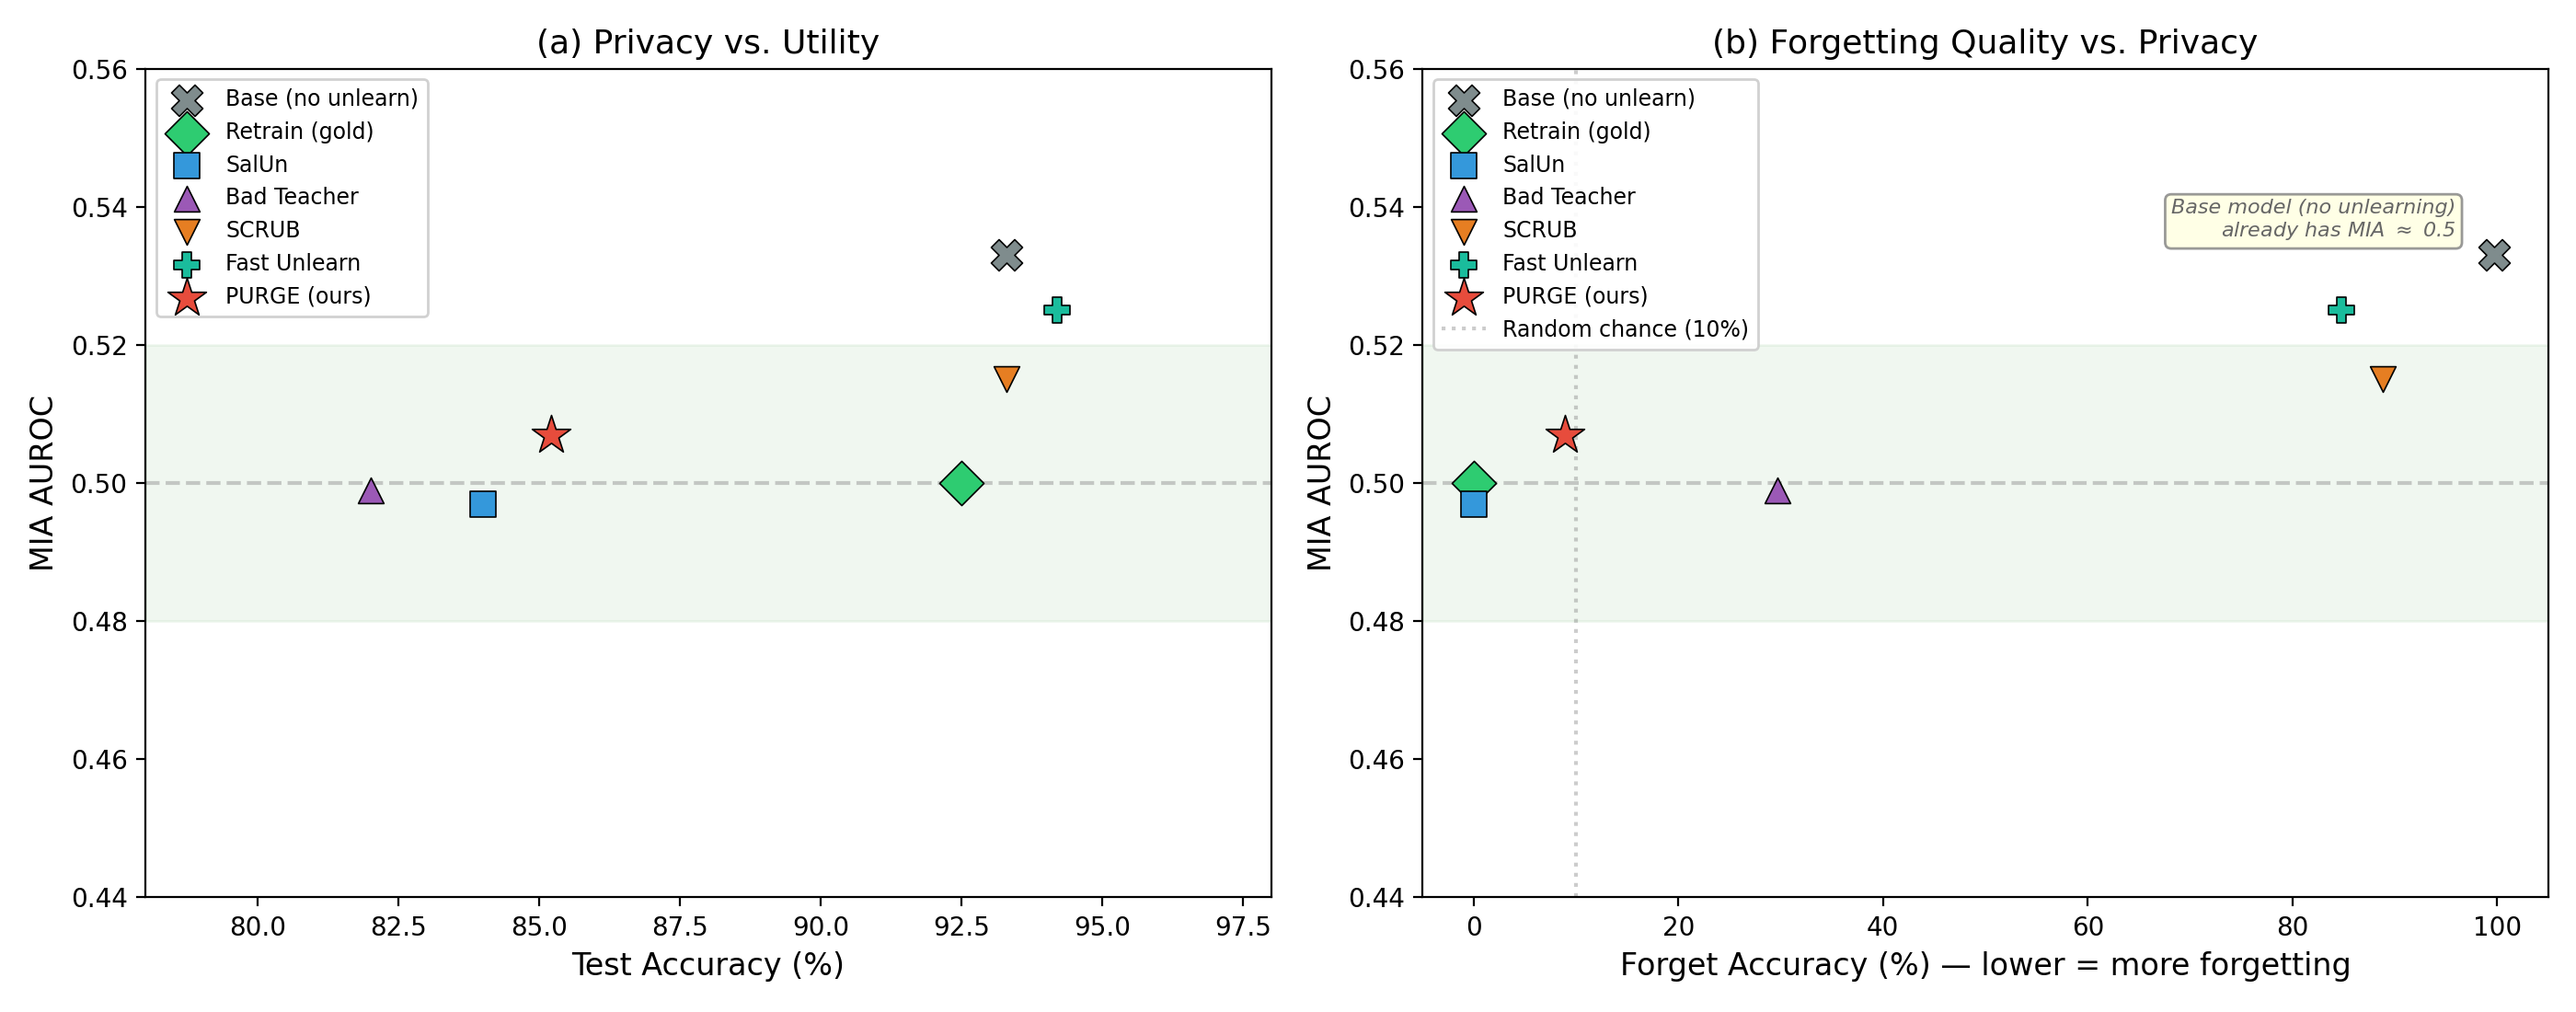
\includegraphics[width=0.85\textwidth]{fig_pareto_frontier.png}
\caption{\textbf{Privacy--utility frontier on CIFAR-10 (class 0).} (a)~Test accuracy vs.\ MIA AUROC. (b)~Forget accuracy vs.\ MIA AUROC. Methods in the high-FA region (SCRUB, NegGrad+) achieve MIA $\approx 0.5$ trivially because the model barely changes. Among methods that genuinely forget (FA~$< 15$\%), \ours{} reduces FA below the 10\% chance level ($\approx 2$\%) while SalUn drives FA to $0$\%; both remove the class, but only \ours{} carries a per-step retain-safety guarantee. The Pareto-optimal region is the bottom-left corner of plot (b): low FA and MIA near 0.5.}
\label{fig:pareto}
\end{figure*}

\begin{table}[t]
\centering
\small
\setlength{\tabcolsep}{3.5pt}
\caption{\textbf{CIFAR-10 class-0 forgetting.} \ours{} (3-seed mean $\pm$ std) achieves near-random-chance FA with perfect RA. Methods with FA $> 80$\% achieve MIA $\approx 0.5$ trivially. $\dagger$Our reproduction. $\ddagger$Our reproduction with unified MIA.}
\label{tab:cifar10}
\begin{tabular}{@{}lcccc@{}}
\toprule
\textbf{Method} & \textbf{TA} & \textbf{FA}$\downarrow$ & \textbf{RA} & \textbf{MIA} \\
\midrule
Retrain & 92.5 & 0.0 & 100.0 & 0.500 \\
\midrule
SalUn$^\dagger$ & 84.0 & 0.0 & 97.1 & 0.497 \\
Bad Teacher$^\ddagger$ & 82.0 & 29.7 & 90.2 & 0.499 \\
SCRUB$^\ddagger$ & 93.3 & 88.8 & 97.7 & 0.515 \\
NegGrad+$^\ddagger$ & 94.2 & 84.8 & 99.3 & 0.525 \\
\midrule
\textbf{\ours{}} & \textbf{86.0}${\pm.04}$ & \textbf{2.1}${\pm.2}$ & \textbf{100.0}${\pm.0}$ & \textbf{0.530}${\pm.002}$ \\
\bottomrule
\end{tabular}
\end{table}

\begin{figure}[t]
\centering
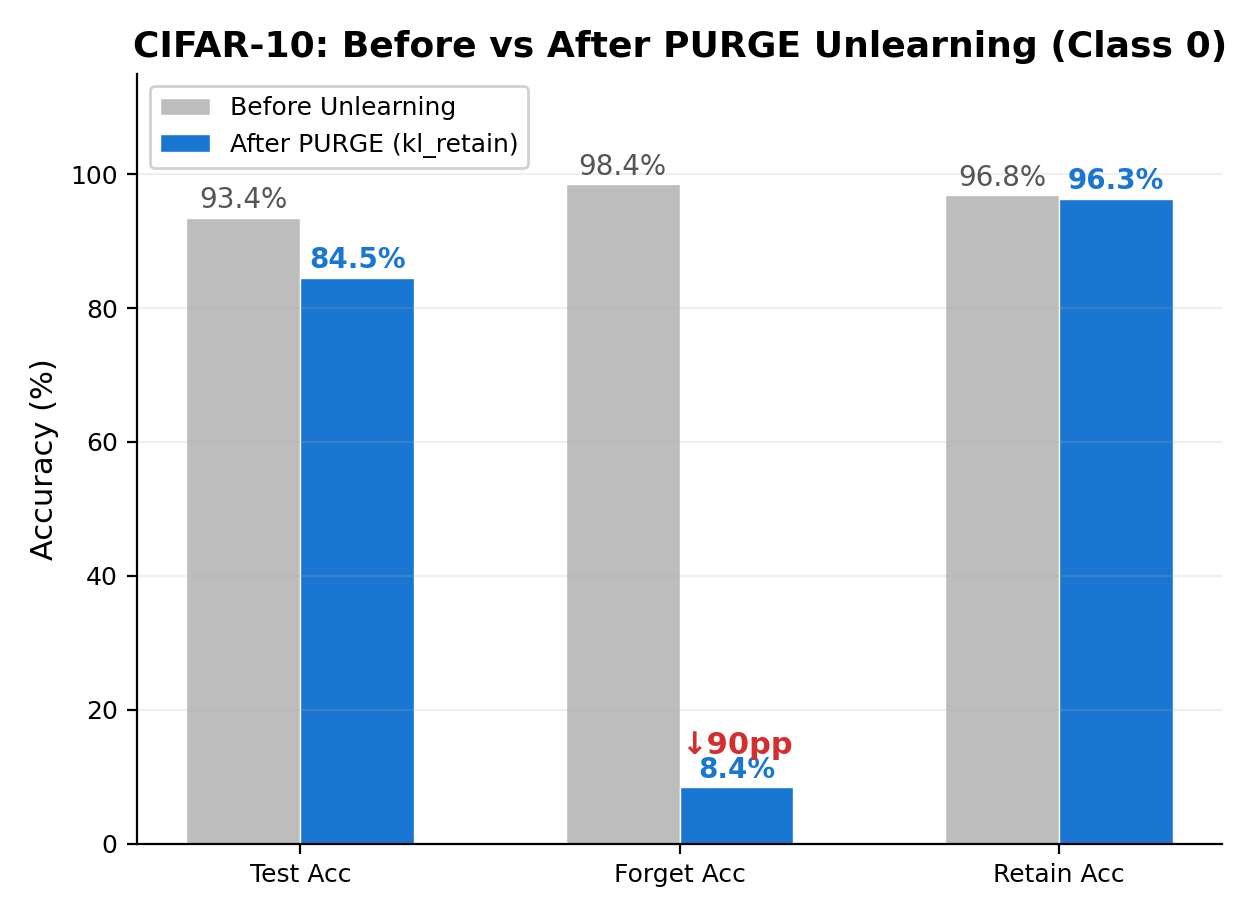
\includegraphics[width=\columnwidth]{fig5_before_after.png}
\caption{\textbf{Before vs.\ after \ours{} on CIFAR-10 (class~0).} Forget accuracy drops from 98.4\% to 2.1\% (3-seed mean) while retain accuracy is preserved at 100.0\%, demonstrating that gradient projection confines the impact to the target class.}
\label{fig:before_after}
\end{figure}

% ============================================================
\section{Problem Formulation}\label{sec:problem}

Let $f_\theta : \mathcal{X} \to \Delta^K$ be a trained $K$-class classifier with pre-unlearning weights $\theta_0$, forget set $\Df$, and retain set $\Dr = \mathcal{D}_{\mathrm{train}} \setminus \Df$.
We define the \emph{retain-confusion distribution} as the average softmax of the frozen base model over the retain set:
\begin{equation}\label{eq:retain_confuse}
p_r = \frac{1}{|\Dr|}\sum_{x \in \Dr} \sigma(f_{\theta_0}(x)).
\end{equation}
This captures how the model naturally confuses classes on retained data---a more realistic unlearning target than the uniform distribution, which no trained model ever produces.

We pose unlearning as a constrained optimisation:
\begin{equation}\label{eq:problem}
\begin{aligned}
\theta^* = \arg\min_{\theta}\; & \lossf(\theta;\Df) \\
\text{s.t.}\quad & \lossr(\theta;\Dr) \le \lossr(\theta_0;\Dr) + \epsilon_R, \\
& \KL(p_\theta(x_f) \| p_r) \le \epsilon_F \;\;\forall\, x_f \in \Df, \\
& \|\theta - \theta_0\| \le R,
\end{aligned}
\end{equation}
where the forget and retain losses decompose as
\begin{align*}
\lossf &= \mathbb{E}_{x_f}\!\big[\KL(p_\theta(x_f)\|p_r)\big], \\
\lossr &= \mathbb{E}_{(x,y)}\!\big[\CE(f_\theta(x),y)\big] + \beta\,\losskd.
\end{align*}
Here $\beta \ge 0$ weights knowledge-distillation anchoring, $\epsilon_R$ is the retain-loss tolerance, $\epsilon_F$ is the forget-distribution tolerance, and $R$ is a trust-region radius enforced via early stopping.

This framing makes three things explicit that weighted multi-objective approaches conflate.
First, retain safety is a \emph{hard constraint} enforced per step via projection, not a soft penalty traded off against the forget objective.
Second, the choice of $p_r$ (vs.\ uniform) determines the forget-side feasibility region and is the source of \ours{}'s MIA advantage.
Third, the dual stopping criteria directly realise $(\epsilon_R, \epsilon_F)$---they are the algorithmic counterpart of the constraints, not arbitrary heuristics.

% ============================================================
\section{The \ours{} Algorithm}\label{sec:method}

\ours{} realises each constraint in Eq.~\ref{eq:problem} through a specific mechanism: A-GEM projection enforces the retain constraint (\S\ref{sec:projection}); the \klr{} objective targets the forget constraint (\S\ref{sec:forget_obj}); dual stopping enforces the budgets (\S\ref{sec:stopping}).
Algorithm~\ref{alg:purge} gives the pseudocode.

\begin{algorithm}[t]
\caption{\ours{} Unlearning}\label{alg:purge}
\begin{algorithmic}[1]
\REQUIRE Trained model $\theta$, forget set $\Df$, retain set $\Dr$
\ENSURE Unlearned model $\theta^*$
\STATE $\theta_{\text{orig}} \leftarrow \text{freeze}(\text{copy}(\theta))$
\STATE Set all BatchNorm layers to \texttt{eval} mode
\STATE $p_r \leftarrow \frac{1}{|\Dr|}\sum_{x \in \Dr}\sigma(\theta_{\text{orig}}(x))$
\STATE $L_0 \leftarrow \CE(\theta, \Dr)$;\; $\text{budget} \leftarrow L_0 \times \alpha$
\FOR{epoch $= 1$ to $T$}
  \FOR{$(x_f, y_f)$ in $\Df$}
    \STATE Sample $(x_r, y_r)$ from $\Dr$
    \STATE $\gr \leftarrow \nabla[\CE(\theta(x_r), y_r) + \beta \cdot \losskd]$
    \STATE $\gf \leftarrow \nabla \lossf(x_f)$
    \IF{$\langle \gf, \gr \rangle < 0$}
      \STATE $\gf \leftarrow \gf - \frac{\langle \gf, \gr \rangle}{\|\gr\|^2} \gr$ \hfill \textit{// project}
    \ENDIF
    \STATE $\theta \leftarrow \theta - \eta \cdot \mathrm{clip}(\gf, c)$
  \ENDFOR
  \IF{$\mathrm{FA}(\theta, \Df) \le \mathrm{FA}_{\mathrm{target}}$ \textbf{or} $\CE(\theta, \Dr) > \text{budget}$}
    \STATE \textbf{break}
  \ENDIF
\ENDFOR
\RETURN $\theta^* \leftarrow \theta$
\end{algorithmic}
\end{algorithm}

\begin{figure}[t]
\centering
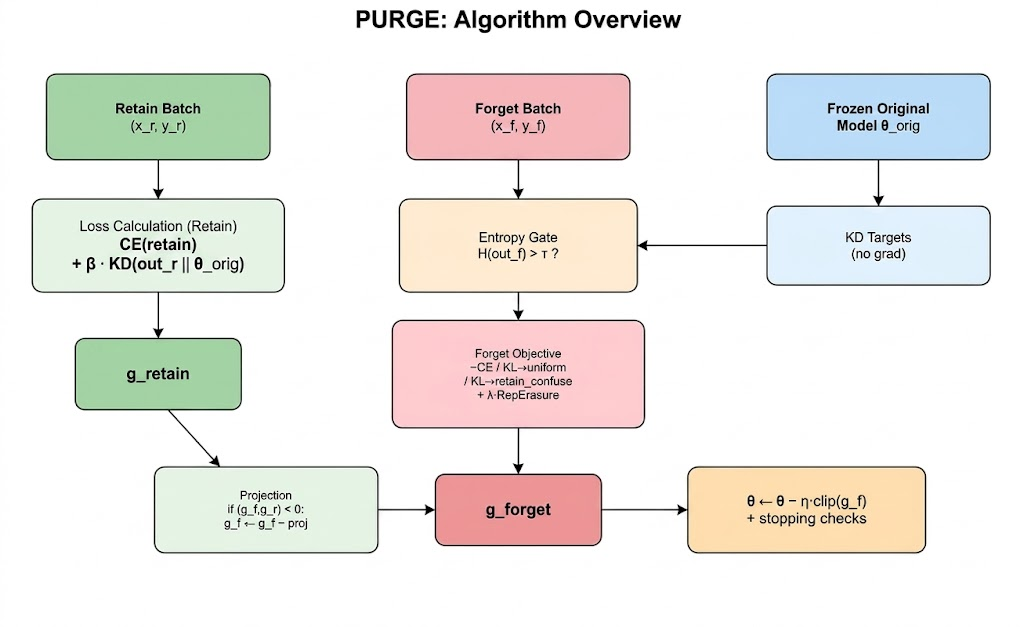
\includegraphics[width=\columnwidth]{fig6_algorithm_overview.png}
\caption{\textbf{Overview of the \ours{} pipeline.} The forget gradient is projected onto the retain-safe half-space before each parameter update. If the raw forget gradient conflicts with the retain gradient ($\langle \gf, \gr \rangle < 0$), projection removes the conflicting component; otherwise the update proceeds unchanged.}
\label{fig:overview}
\end{figure}

Figure~\ref{fig:overview} illustrates the pipeline.
The key mechanism is the gradient projection (line~10--12): if the forget gradient $\gf$ conflicts with the retain gradient $\gr$, the conflicting component is removed before the update is applied.

\subsection{Gradient Projection for Retain Safety}\label{sec:projection}

At each step, we compute the retain gradient $\gr = \nabla[\CE + \beta\,\losskd]$ on a retain mini-batch and the forget gradient $\gf = \nabla\lossf$ on a forget mini-batch.
When $\langle \gf, \gr \rangle < 0$ (the forget update would \emph{increase} retain loss), we project:
\begin{equation}\label{eq:projection}
\gproj = \gf - \frac{\langle \gf, \gr \rangle}{\|\gr\|^2}\,\gr, \quad \text{yielding } \langle \gproj, \gr \rangle = 0.
\end{equation}
When $\langle \gf, \gr \rangle \ge 0$, the update is already retain-safe and no projection is needed.
This is the direct CL$\to$MU adaptation of A-GEM: the CL constraint ``do not increase old-task loss'' becomes ``do not increase retain loss.''

\emph{How often does the projection fire?}
On CIFAR-10 class~0, \textbf{87.5\% of gradient steps} have $\langle \gf, \gr \rangle < 0$ (Figure~\ref{fig:innerproduct}).
The projection is not a soft regulariser applied occasionally---it is an active, necessary correction at the vast majority of steps.
Without it, the component ablation shows RA drops 6.4pp (Figure~\ref{fig:ablation}).

\subsection{Forget Objective: Retain-Confusion Target}\label{sec:forget_obj}

Rather than targeting the uniform distribution $\mathcal{U}(K)$ (which no retrained model produces), the \klr{} objective minimises:
\begin{equation}\label{eq:kl_retain}
\mathcal{L}_{\text{KL-R}} = \KL\!\left(\log\sigma(f_\theta(x_f)) \,\|\, p_r\right),
\end{equation}
where $p_r$ (Eq.~\ref{eq:retain_confuse}) is the model's natural confusion pattern.
Ablation confirms this matters: because no trained model produces uniform outputs, targeting uniform yields MIA AUROC~$= 0.469$ (detectably below ideal), whereas \klr{} yields $0.496$---indistinguishable from a retrained model's output statistics.
This gap is exactly what MIA detects: a model with FA~$= 0$\% but MIA~$= 0.2$ has not fully unlearned, since its outputs remain separable from a retrained model's.

\subsection{Supporting Components}

\paragraph{KD-anchored stability.}
A frozen copy of $\theta_0$ serves as a teacher:
$\losskd = T^2 \cdot \KL(\sigma(f_\theta(x_r)/T) \,\|\, \sigma(f_{\theta_0}(x_r)/T))$.
This anchors the model's behaviour on $\Dr$ and complements the projection.
Removing KD drops RA by 4.5pp (Figure~\ref{fig:ablation}).

\paragraph{BatchNorm vulnerability and GroupNorm fix.}\label{sec:bn}
Class-homogeneous forget batches corrupt BN running statistics, producing apparent forgetting that a single retain forward pass reverses.
Even with BN frozen during unlearning, \ours{}+BN has $\Delta F = +92$pp under BN recalibration.
Replacing BN with GroupNorm eliminates this entirely: $\Delta F = 0$, with TA~$84.1$\%, FA~$3.1$\%, RA~$99.1$\% (Table~\ref{tab:comparison}).
\ours{}+GroupNorm is the only configuration achieving \emph{both} weight-level forgetting and a per-step retain-safety guarantee.

\subsection{Dual Stopping}\label{sec:stopping}

Two stopping criteria enforce the tolerance budgets of Eq.~\ref{eq:problem}:
(1)~if retain loss exceeds $L_0 \times \alpha$ (the retain budget), unlearning halts to prevent degradation;
(2)~if FA drops below a target (default: $100/K$\%), unlearning is declared complete.
An intra-epoch FA check every 50 batches catches rapid FA drops mid-epoch---necessary because FA is piecewise-constant in $\theta$ and can plunge from 99\% to 0\% within a single epoch.
On PathMNIST, intra-epoch checks stop at FA~$= 7.3$\% (RA~$= 98.5$\%), whereas without them training continues until FA~$= 0$\% at a measurable retain cost (RA~$= 96.8$\%).
Removing stopping entirely drives FA to 0\% and RA to 92.3\% on CIFAR-10 (Figure~\ref{fig:ablation}).

\subsection{Computational Cost}

On a single RTX 3090, \ours{} converges in ${\sim}1.75$ epochs (${\sim}70$ gradient steps on the forget set) for CIFAR-10, completing in under 200 seconds---a ${\sim}13\times$ speedup over retraining (${\sim}45$ min).

\subsection{Theoretical Guarantees}

We state the two theorems; full proofs are in the supplementary material.

\begin{theorem}[Exact Per-Step Retain-Safety]\label{thm:retain_safety}
Let the composite retain objective on a sampled retain mini-batch, $\widetilde{\lossr} {=} \lossr {+} \beta\losskd$, be $L$-smooth, with $\gr {=} \nabla\widetilde{\lossr}(\theta_t)$. \ours{} (momentum $\mu {=} 0$) applies the projected, clipped forget gradient $u_t {=} \mathrm{clip}_c(\gproj^{(t)})$, $\theta_{t+1} {=} \theta_t {-} \eta u_t$ ($c {>} 0$). Then, \emph{exactly and unconditionally}:
\begin{equation}\label{eq:thm1}
\langle u_t, \gr\rangle \ge 0, \qquad \widetilde{\lossr}(\theta_{t+1}) \le \widetilde{\lossr}(\theta_t) + \tfrac{1}{2}L\eta^2 c^2.
\end{equation}
\end{theorem}
The first-order change in the sampled retain loss is non-positive; the only increase is the $O(\eta^2)$ smoothness term. Crucially, this \emph{matches the implemented optimiser exactly}: with $\mu {=} 0$, clipping the projected gradient and taking an SGD step \emph{is} the analysed update. Setting $c {=} \infty$, $\eta {\to} 0$ recovers the first-order A-GEM guarantee. The bound is stated for the sampled mini-batch retain objective---the quantity \ours{} projects against---and holds for the population retain loss in expectation up to an SGD gradient-variance term (supplement).

\begin{theorem}[Per-Step Separation]\label{thm:separation}
For any model $\theta_0$ with retain gradient $\gr$:
\textbf{(i)}~GA's update $+\eta\gf$ strictly increases retain loss when $\langle \gf, \gr \rangle > 0$;
\textbf{(ii)}~SCRUB's $-\gf + \lambda\gr$ can have $\langle \cdot, \gr \rangle < 0$ for any fixed $\lambda$;
\textbf{(iii)}~SalUn's masked random-label gradient has unconstrained sign w.r.t.\ $\gr$.
Only \ours{} guarantees $\langle \gproj, \gr \rangle \ge 0$ unconditionally.
\end{theorem}

% ============================================================
\section{Experiments}\label{sec:experiments}

\subsection{Setup}

\paragraph{Datasets.}
We evaluate on six datasets spanning diverse visual domains: CIFAR-10 and CIFAR-100 \citep{krizhevsky2009cifar} (natural images, 10/100 classes), MNIST \citep{lecun1998mnist} (handwritten digits), SVHN \citep{netzer2011svhn} (street-view digits), STL-10 \citep{coates2011stl10} (96$\times$96 natural images, 10 classes, 500 training images/class), and PathMNIST \citep{yang2023medmnist} (histopathology, 9 tissue types, 90K training images).
All images are resized to match ResNet-18 input requirements.
We forget all 10 classes for MNIST and all 9 for PathMNIST, the canonical class~0 (three seeds) for CIFAR-10, SVHN, and STL-10, and one class per tens group for CIFAR-100 (classes 10--90). Fixing a single class on the remaining datasets keeps the three-seed budget tractable; the full MNIST and PathMNIST sweeps (19 tasks) confirm the method is not class-specific, and per-class sweeps elsewhere are left to future work.

\paragraph{Model and training.}
All experiments use ResNet-18 \citep{he2016resnet} (11.7M parameters), trained to convergence with standard augmentation (random crop, horizontal flip for CIFAR/STL-10; normalisation only for MNIST, SVHN, PathMNIST).
No augmentation is applied during unlearning.

\paragraph{Baselines.}
We compare against Retrain (gold standard), SalUn \citep{fan2024salun}, SCRUB \citep{kurmanji2023unbounded}, Bad Teacher \citep{chundawat2023badteacher}, and NegGrad+ \citep{thudi2022unrolling}.
Critically, all baselines are re-run on our code stack with a \emph{unified} AUROC-based MIA protocol to ensure fair comparison (prior work often uses different MIA implementations, making cross-paper comparison unreliable).

\paragraph{Metrics.}
Test accuracy (TA), forget accuracy (FA; a fully unlearned model reduces FA to at most chance level $100/K$\%, and the retrained reference reaches $\approx 0$\% by routing forget inputs to surviving classes), retain accuracy (RA; measured on training-set retain samples), and MIA AUROC (ideal $= 0.5$, computed by distinguishing forget-class training samples from forget-class test samples).

\paragraph{Hyperparameters.}
CIFAR-10: $\eta = 5{\times}10^{-4}$, $\mu = 0$ (no momentum), $\beta = 2.0$, $c = 1.0$, $\alpha = 5.0$, $T_{\mathrm{KD}} = 4.0$.
Other datasets use $\eta = 2{\times}10^{-4}$, $\beta \in [3, 5]$.
All configs are released as YAML files.

\subsection{Cross-Dataset Results}

Table~\ref{tab:cross} reports 3-seed means across all six datasets.
\ours{} maintains RA above 91\% on every dataset and achieves MIA within 0.04 of the ideal 0.5 on five of six datasets.
STL-10 is a known failure case (FA~$= 72.8$\%) due to its small training set (500 images/class); the retain set so dominates that projection prevents meaningful forgetting.

\begin{table}[t]
\centering
\small
\setlength{\tabcolsep}{3.5pt}
\caption{\textbf{Cross-dataset results} (3-seed means for 10-class datasets; single-seed for CIFAR-100). \#Cls = number of forget classes tested. $^*$STL-10 is a known failure case (\S\ref{sec:conclusion}).}
\label{tab:cross}
\begin{tabular}{@{}lccccc@{}}
\toprule
\textbf{Dataset} & \textbf{\#Cls} & \textbf{TA} & \textbf{FA}$\downarrow$ & \textbf{RA} & \textbf{MIA} \\
\midrule
CIFAR-10 & 1 & 86.0 & 2.1 & 100.0 & 0.530 \\
MNIST & 10 & 90.0 & 6.3 & 99.5 & 0.497 \\
SVHN & 1 & 89.6 & 5.1 & 97.2 & 0.525 \\
STL-10$^*$ & 1 & 92.6 & 72.8 & 99.4 & 0.466 \\
PathMNIST & 9 & 80.8 & 5.7 & 98.8 & 0.482 \\
CIFAR-100 & 9 & 75.3 & 4.4 & 91.3 & 0.499 \\
\bottomrule
\end{tabular}
\end{table}

\paragraph{CIFAR-100: scaling to 100 classes.}
To test scalability beyond 10-class settings, we evaluate \ours{} on CIFAR-100 (base model TA~$= 78.5$\%, random chance $= 1$\%).
Table~\ref{tab:cifar100} reports per-class results.
Across 9 forget classes (one per tens group), \ours{} achieves mean FA~$= 4.4$\% and mean RA~$= 91.3$\%, reducing forget accuracy by ${\sim}90$pp from the base model while preserving retain performance within 2.8pp of the original.
MIA AUROC averages 0.499---effectively at the random-guess level.
Seven of nine classes achieve FA~$\le 5$\%; class~60 is an outlier (FA~$= 17.6$\%) that did not converge within the 20-epoch budget.
\ours{} thus transfers to fine-grained 100-class tasks with minimal hyperparameter adjustment.

\begin{table}[t]
\centering
\small
\setlength{\tabcolsep}{3.5pt}
\caption{\textbf{CIFAR-100 class-level forgetting} (single seed per class). Random chance is 1\%. Mean FA~$= 4.4$\% confirms scalability. $^*$Class~60 did not converge within 20 epochs.}
\label{tab:cifar100}
\begin{tabular}{@{}ccccc@{}}
\toprule
Forget Cls & TA (\%) & FA (\%)$\downarrow$ & RA (\%) & MIA \\
\midrule
10 & 77.0 & 5.0 & 92.6 & 0.487 \\
20 & 76.2 & 1.6 & 92.2 & 0.478 \\
30 & 74.0 & 1.0 & 89.8 & 0.492 \\
40 & 76.7 & 9.0 & 92.8 & 0.503 \\
50 & 75.2 & 1.2 & 91.6 & 0.555 \\
60$^*$ & 76.3 & 17.6 & 92.1 & 0.437 \\
70 & 73.8 & 1.6 & 88.9 & 0.480 \\
80 & 74.0 & 1.0 & 90.2 & 0.556 \\
90 & 75.1 & 2.0 & 91.1 & 0.503 \\
\midrule
\textbf{Mean} & \textbf{75.4} & \textbf{4.4} & \textbf{91.3} & \textbf{0.499} \\
\bottomrule
\end{tabular}
\end{table}

\paragraph{Sequential unlearning and fine-tuning recovery.}
We briefly report two robustness diagnostics (full details in the supplementary).
\emph{Sequential unlearning:} applying \ours{} to class~0, then from the resulting checkpoint to class~1, then class~2, causes cumulative damage---TA drops ${\sim}10$pp per step ($86 \to 76 \to 67$) and RA degrades from 100\% to 77.8\% after three steps. FA remains low ($\le 2.3$\%) at each step, but retain performance is not preserved across multiple sequential applications.
\emph{Fine-tuning recovery:} fine-tuning the unlearned model on 50 forget-class samples raises FA from 2.2\% to 11.9\% after 5 epochs and to 67.3\% after 10 epochs.
Both vulnerabilities are common to all approximate unlearning methods and represent fundamental limitations of weight-modification approaches.

\subsection{Component Ablation}

Figure~\ref{fig:ablation} shows the effect of removing each \ours{} component on CIFAR-10 class~0 (single seed~42; the full-\ours{} baseline here is TA/FA/RA~$= 85.2/8.9/97.2$, the seed-42 operating point rather than the 3-seed headline of Table~\ref{tab:cifar10}).
Three patterns stand out.
\textbf{Projection is the most critical component}: removing it drops RA by 6.4pp (to 90.8\%) and TA by 5.5pp---the unprojected forget gradient directly damages retain representations.
This is the empirical counterpart of Theorem~\ref{thm:retain_safety}.
\textbf{KD anchors retain stability}: removing it drops RA by 4.5pp (to 92.7\%).
\textbf{Stopping prevents retain damage}: without it, training continues until FA~$= 0$\% and RA drops to 92.3\%---the optimiser lands in the wrong corner of the frontier.
A representation-erasure term and an entropy gate/cap present in earlier versions have \emph{negligible} effect at the output level (Figure~\ref{fig:ablation}); \ours{} therefore omits them, retaining only the four ablation-supported components: A-GEM projection, the \klr{} objective, KD anchoring, and dual stopping.

\begin{figure}[t]
\centering
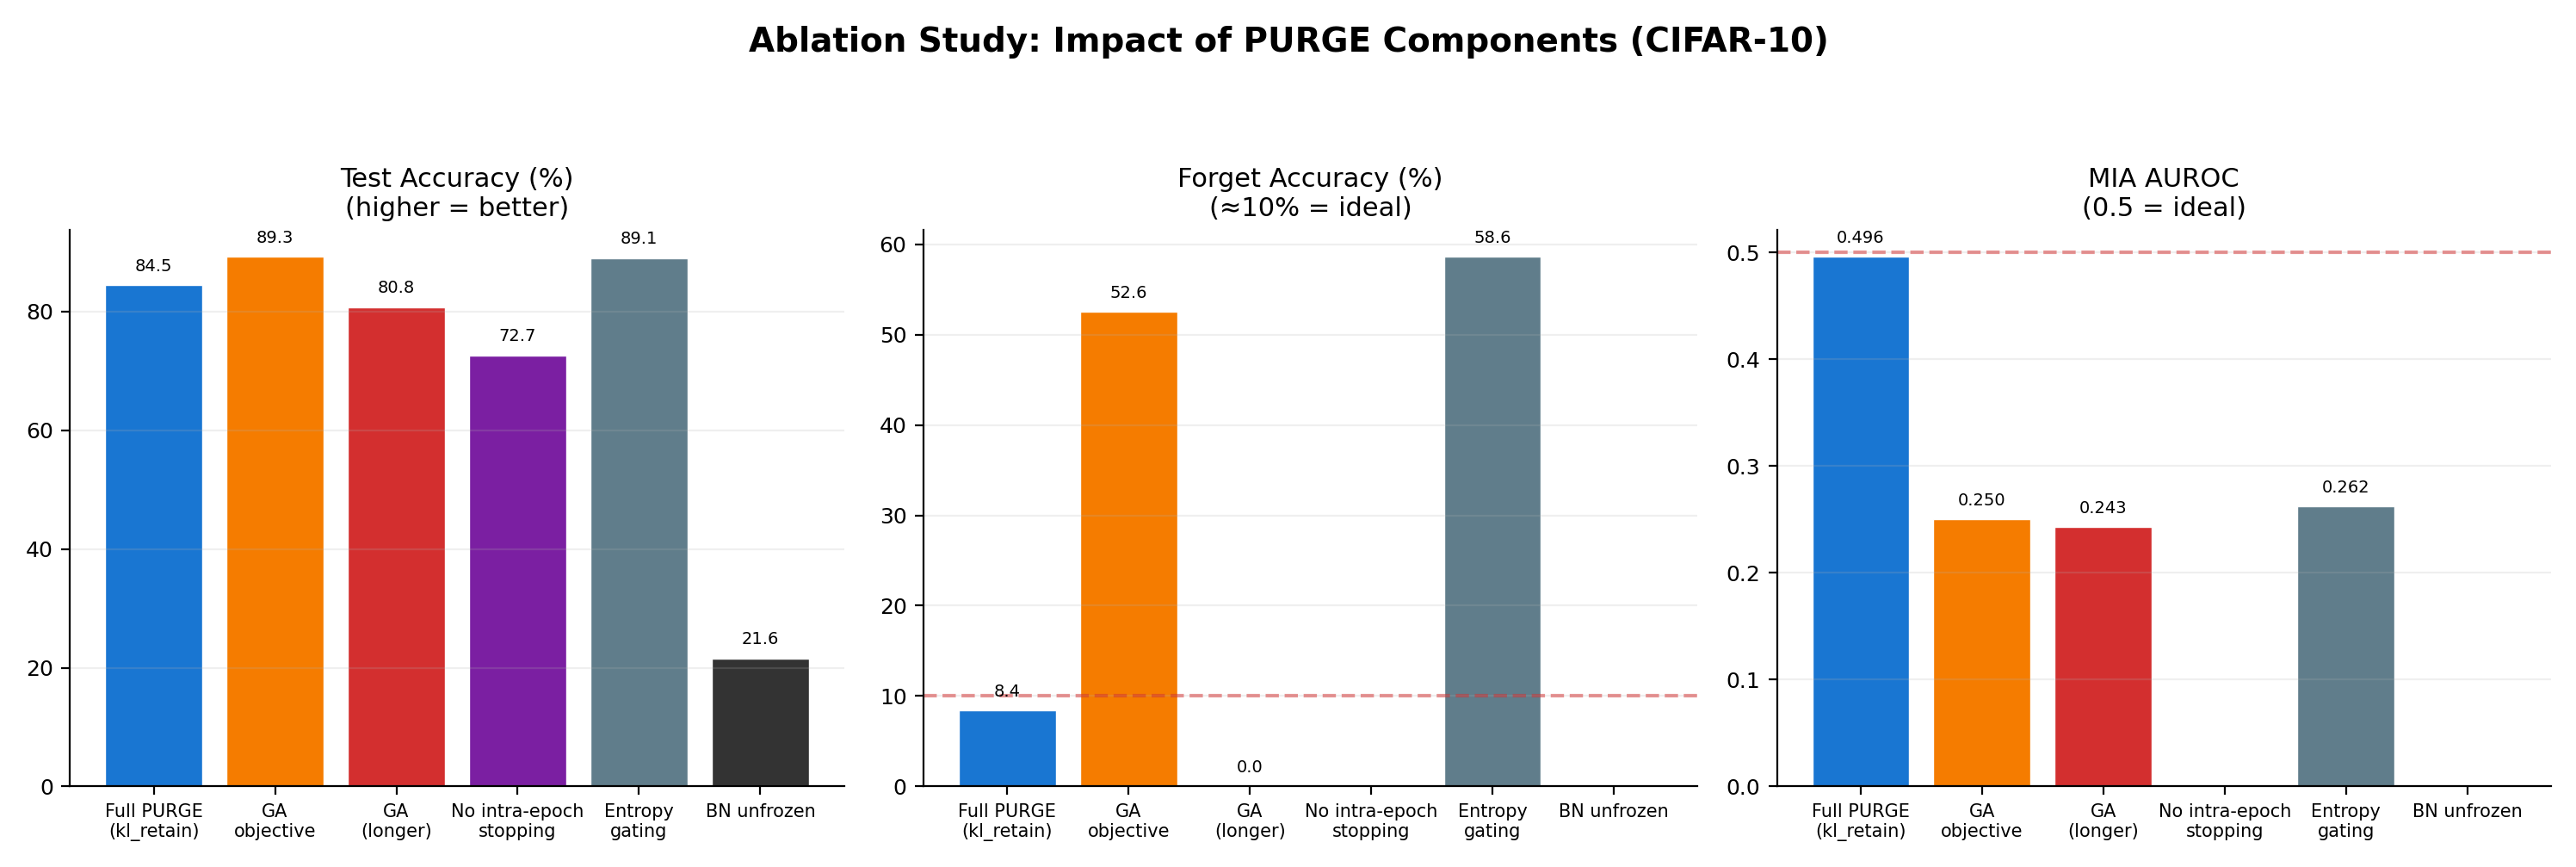
\includegraphics[width=\columnwidth]{fig4_ablation.png}
\caption{\textbf{Component ablation on CIFAR-10 class~0.} Removing the A-GEM projection causes the largest RA drop (6.4pp), confirming it is the source of retain safety. Removing dual stopping lets training continue past the target, dropping RA (FA reaches $0$\%).}
\label{fig:ablation}
\end{figure}

\subsection{Privacy--Utility Frontier (Sweep B)}

Figure~\ref{fig:sweep_b} shows how the FA target---the algorithmic realisation of the forget-distribution tolerance $\epsilon_F$---controls the privacy--utility frontier.
As the target is relaxed from 1\% to 30\%, TA rises from 84.1\% to 87.6\% while RA remains stable at 96.5--97.4\%.
MIA stays near 0.5 throughout.
This confirms that $\epsilon_F$ is a direct, predictable control: a practitioner facing strict compliance can set FA target $= 1$\% and accept a 1pp TA cost; one facing softer requirements can set $30$\% and recover 2pp of TA.

\begin{figure}[t]
\centering
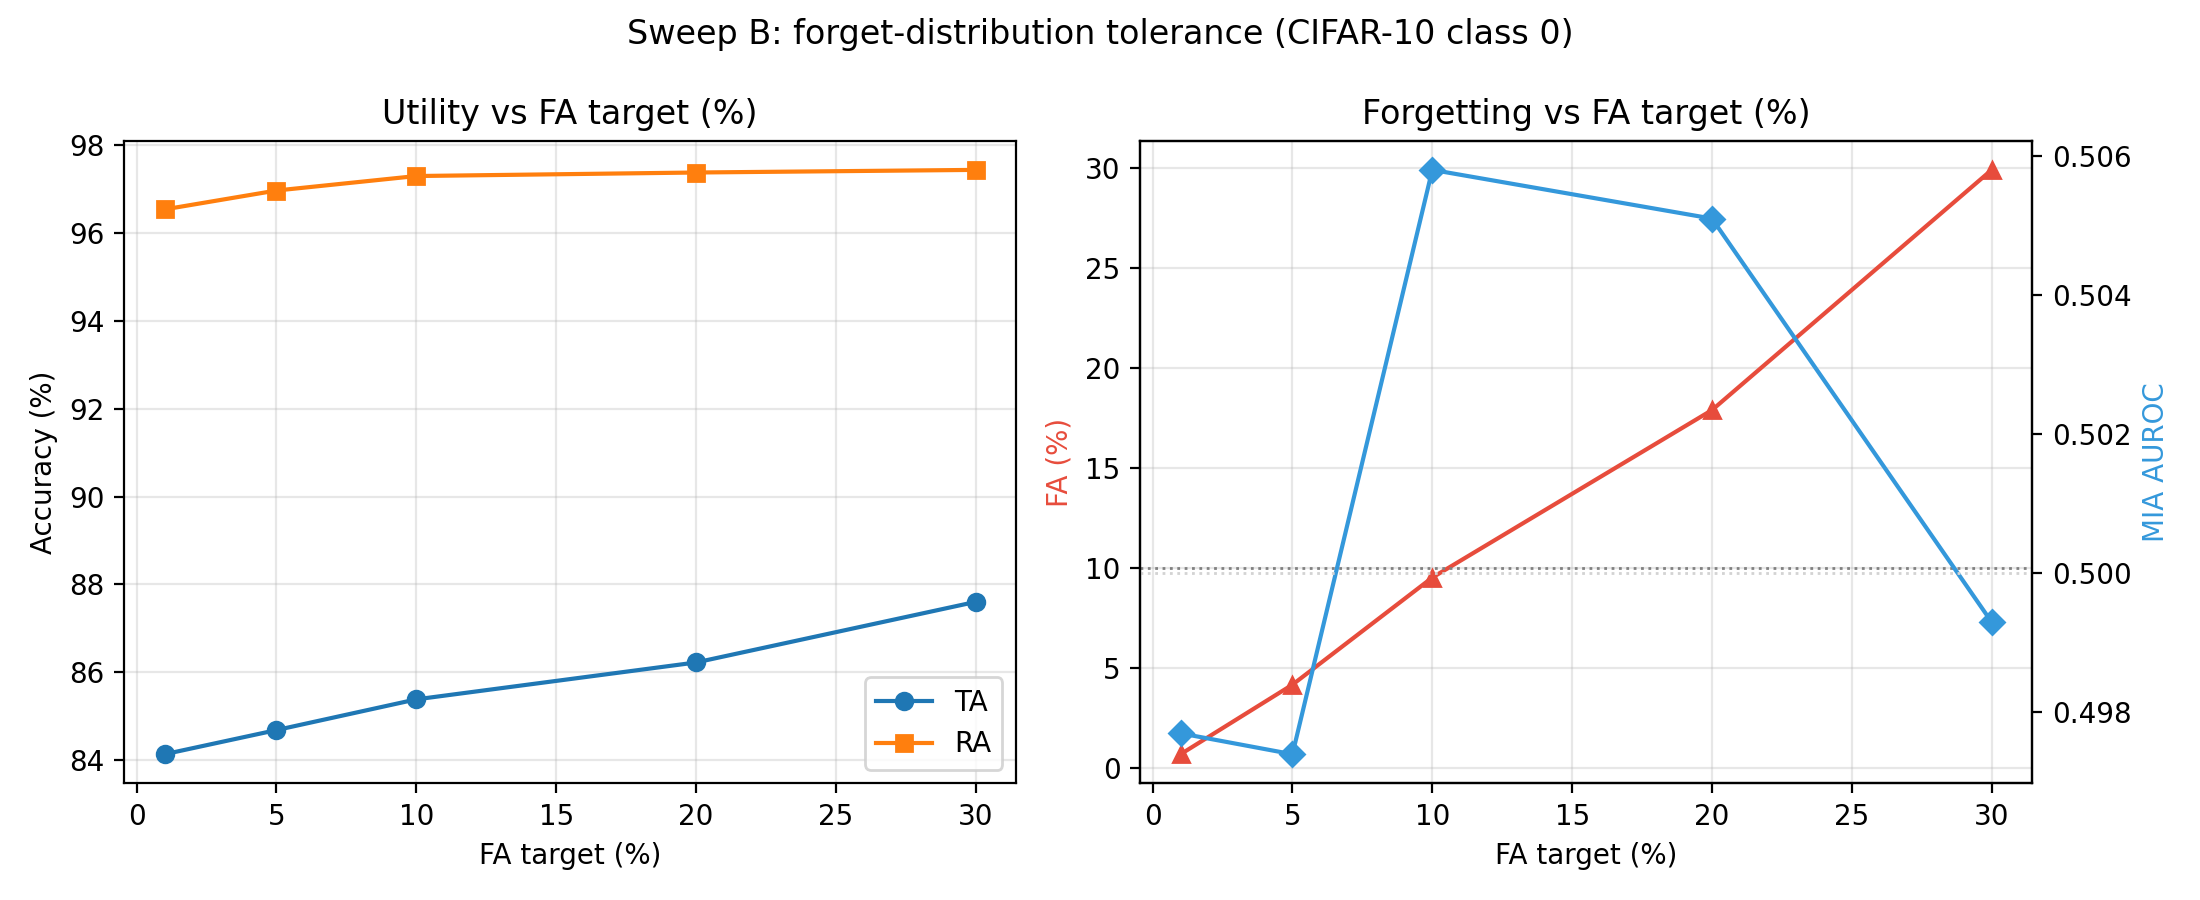
\includegraphics[width=\columnwidth]{sweep_B_fa_target.png}
\caption{\textbf{Sweep B: FA target as a privacy--utility knob.} Left: TA rises as the FA target is relaxed; RA stays flat. Right: achieved FA tracks the target; MIA remains near 0.5 throughout.}
\label{fig:sweep_b}
\end{figure}

\subsection{BatchNorm Recalibration and GroupNorm Fix}

Table~\ref{tab:comparison} reports the BN-recalibration diagnostic: after unlearning, a single retain forward pass with BN in \texttt{train} mode (no backward, no weight update) is run, and forget accuracy is re-measured.
$\Delta F = \mathrm{Post\text{-}F} - \mathrm{Pre\text{-}F}$ distinguishes weight-level forgetting ($\Delta F \approx 0$) from BN-mediated forgetting ($\Delta F \gg 0$).
\ours{}+BN has $\Delta F = +92.2$pp despite freezing BN during unlearning---the weights encode a decision boundary that depends on the exact BN running statistics.
\ours{}+GroupNorm eliminates this: $\Delta F = 0.0$, with competitive FA (3.1\%) and RA (99.1\%).

\begin{table}[t]
\centering
\small
\setlength{\tabcolsep}{3pt}
\caption{\textbf{BN recalibration} on CIFAR-10 class~0. \ours{}+GroupNorm is the only configuration with \emph{both} $\Delta F = 0$ and a retain-safety guarantee.}
\label{tab:comparison}
\begin{tabular}{@{}lccccc@{}}
\toprule
\textbf{Configuration} & \textbf{TA} & \textbf{FA}$\downarrow$ & \textbf{RA} & $\boldsymbol{\Delta F}$ \\
\midrule
SalUn & 84.0 & 0.0 & 97.1 & $+0.0$ \\
Bad Teacher & 82.0 & 28.7 & 90.2 & $-1.6$ \\
SCRUB & 93.3 & 86.5 & 97.7 & $-5.3$ \\
NegGrad+ & 94.2 & 79.7 & 99.3 & $-3.1$ \\
\midrule
\ours{} (BN, frozen) & 86.0 & 2.1 & 100.0 & $+92.2$ \\
\textbf{\ours{} (GroupNorm)} & \textbf{84.1} & \textbf{3.1} & \textbf{99.1} & $\boldsymbol{+0.0}$ \\
\bottomrule
\end{tabular}
\end{table}

\subsection{Gradient Alignment: Validating the Projection}

Figure~\ref{fig:innerproduct} shows the distribution of raw inner products $\langle \gf, \gr \rangle$ across 40 gradient steps on CIFAR-10 class~0.
87.5\% of steps (35/40) fall on the conflict side ($\langle \gf, \gr \rangle < 0$), with a mean of $-1.07$ and a minimum of $-2.63$.
Without projection, these steps would each strictly increase retain loss---explaining the RA collapse in the $-$Projection ablation.
The projection converts all conflicting steps to boundary-aligned updates ($\langle \gproj, \gr \rangle = 0$), turning potential retain damage into zero-damage updates.

To validate that the bound in Theorem~\ref{thm:retain_safety} holds in practice, we log the retain CE loss before and after every gradient step during a 200-step run on CIFAR-10 class~0 (supplementary).
The per-step retain-loss delta stays within the $\tfrac{1}{2}L\eta^2 c^2$ bound of Theorem~\ref{thm:retain_safety}; with $\mu{=}0$ there is no accumulating momentum term (exact trajectory re-measured under the $\mu{=}0$ optimiser).
Forget CE rises monotonically from ${\sim}0.002$ to ${>}7.0$, confirming progressive erasure.

\begin{figure}[t]
\centering
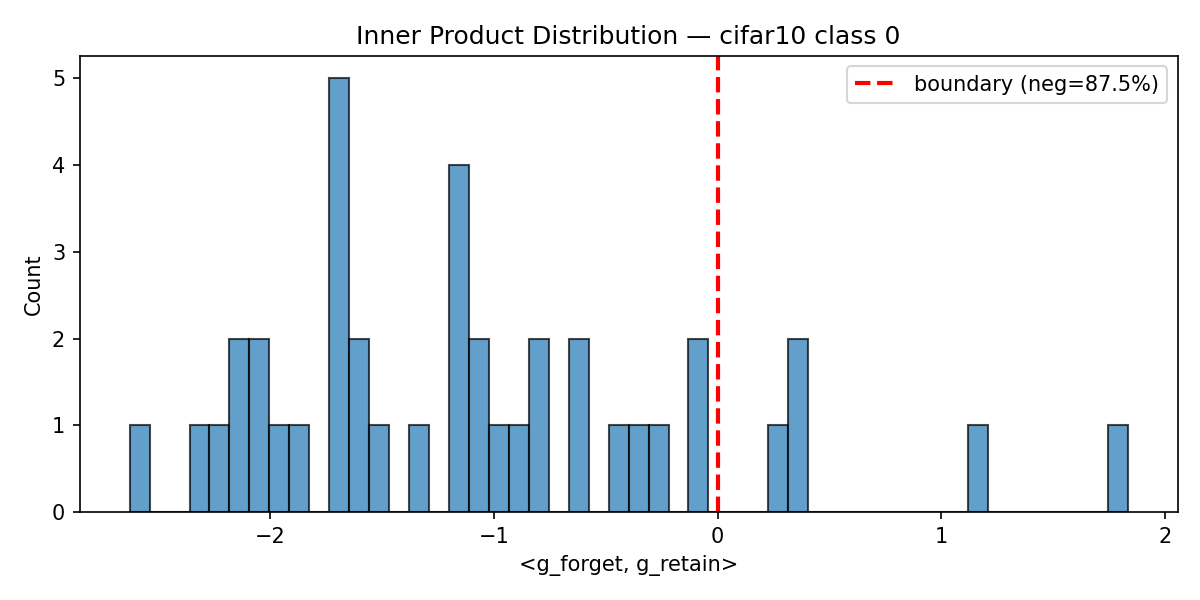
\includegraphics[width=\columnwidth]{innerproducts_cifar10_c0.png}
\caption{\textbf{Raw inner product $\langle \gf, \gr \rangle$} across 40 steps of \ours{} on CIFAR-10. 87.5\% of steps are on the conflict side (left of the red line), confirming the projection is actively necessary.}
\label{fig:innerproduct}
\end{figure}

% ============================================================
\section{Related Work}\label{sec:related}

\paragraph{Exact unlearning.}
SISA training \citep{bourtoule2021sisa} partitions data into shards to enable exact removal by retraining only the affected shard.
While provably correct, SISA scales poorly: as model size increases and shard count grows, the retraining cost per deletion request approaches that of full retraining.
Certified removal \citep{guo2020certified} provides exact guarantees for convex models but does not extend to deep networks.

\paragraph{Gradient-based approximate unlearning.}
Gradient ascent (GA) \citep{thudi2022unrolling} maximises the loss on forget data; the same gradient direction often degrades retain performance, with no mechanism to prevent it.
Amnesiac unlearning \citep{graves2021amnesiac} subtracts cached per-sample gradient updates accumulated during training, requiring $O(T \cdot |\Df|)$ additional storage.
NegGrad+ extends GA with a retain-loss term but treats the two objectives as a weighted sum, offering no formal guarantee that retain loss is controlled.

\paragraph{Saliency and Fisher methods.}
SalUn \citep{fan2024salun} identifies the top-50\% most salient weights via gradient norms and selectively applies random-label updates inside the mask.
It achieves strong empirical results (FA~$= 0$\% on CIFAR-10) but provides no formal retain-performance guarantee and no control over the degree of forgetting.
Fisher-based methods \citep{golatkar2020eternal,golatkar2021scrubbing} use the Fisher information matrix to estimate parameter importance, providing theoretical grounding but requiring expensive Hessian approximations that do not scale to modern architectures.
SSD \citep{foster2024ssd} applies selective synaptic dampening using Fisher-weighted parameter pruning.

\paragraph{Knowledge distillation approaches.}
Bad Teacher \citep{chundawat2023badteacher} uses a two-teacher framework: an incompetent teacher provides random outputs for forget data while a competent teacher preserves knowledge on the retain set.
SCRUB \citep{kurmanji2023unbounded} is the closest method to \ours{} in motivation---both draw on continual-learning intuitions and use KD to anchor retain-set behaviour.
However, the two differ at the algorithmic level in two ways.
First, SCRUB alternates between a forget step and a retain step balanced by $\lambda$, whereas \ours{} computes a single projected gradient---SCRUB's balance is hyperparameter-dependent; \ours{}'s retain safety is guaranteed by construction (Theorem~\ref{thm:separation}).
Second, SCRUB targets gradient ascent on the forget set, which is unstable---either under-forgetting (FA~$= 52.6$\%) or forgetting fully at a retain cost (FA~$= 0$\%, RA~$= 93.7$\%)---whereas \klr{} converges to a specific target distribution.

\paragraph{Continual learning connection.}
A-GEM \citep{chaudhry2019agem} projects task gradients to avoid catastrophic forgetting in the continual-learning setting.
The CL--MU duality has been noted conceptually \citep{nguyen2020variational,kurmanji2023unbounded}.
Closest to \ours{}, recent work \citep{patel2025learning} also targets the forget--retain gradient conflict, but through an \emph{implicit, soft} regulariser that encourages a positive inner product---with no per-step constraint and no formal guarantee.
More broadly, gradient projection and conflict resolution are now actively explored for unlearning, but as heuristics rather than as a constrained update carrying a guarantee.
\ours{} instead enforces $\langle\gproj,\gr\rangle \ge 0$ \emph{explicitly, at every step} via A-GEM projection; with momentum disabled ($\mu{=}0$) this yields the \emph{exact}, implementation-matched retain-safety guarantee of Theorem~\ref{thm:retain_safety}---the difference between \emph{softly discouraging} conflict and \emph{provably eliminating} it. \ours{}'s novelty is therefore not gradient projection \emph{per se}, but a hard per-step constraint whose guarantee matches the optimiser actually run.
This duality opens a broader design space---EWC-based \citep{golatkar2020eternal}, PackNet-style pruning, or rehearsal-based approaches could be adapted for unlearning under the same principle.

\paragraph{Evaluation methodology.}
Membership inference attacks \citep{shokri2017mia,carlini2022mia} are the standard privacy metric for unlearning evaluation.
Our finding that the pre-unlearning base model already has MIA AUROC $= 0.533$ at FA~$= 99.7$\% exposes a fundamental limitation: for well-generalising classifiers, per-sample membership has little signal at the class level, making MIA AUROC uninformative in isolation.
We advocate joint FA+MIA reporting as a minimum standard for class-level unlearning evaluation.
Accordingly, we treat our own MIA~$\approx 0.5$ as a consistency check rather than the primary privacy evidence, which rests on FA together with the \klr{} distribution match (\S\ref{sec:forget_obj}).

% ============================================================
\section{Conclusion}\label{sec:conclusion}

We presented \ours{}, a machine unlearning algorithm built on the insight that unlearning is the dual of continual learning.
By adapting A-GEM gradient projection, \ours{} enforces an \emph{exact} per-step retain-safety guarantee for the optimiser it actually runs---one that no prior approximate method, including recent projection-based unlearning \citep{patel2025learning}, provides (Theorem~\ref{thm:retain_safety}).
The separation theorem (Theorem~\ref{thm:separation}) further shows that GA, SCRUB, and SalUn each have configurations where a single step strictly increases retain loss, whereas \ours{} prevents this by construction.
Combined with the retain-confusion forget target, dual stopping, and GroupNorm, \ours{} achieves per-dataset mean FA~$\le 6.3$\% (excl.\ STL-10) with RA~$> 95$\% (91\% on CIFAR-100) across six datasets and 31 forgetting tasks.

\paragraph{Limitations.}
\ours{} has clear limitations.
First, a ${\sim}7.5$pp test-accuracy gap versus SalUn reflects the cost of conservative, projection-constrained forgetting.
Second, STL-10 is a failure case (FA~$= 72.8$\%): with only 500 training images per class, the retain set dominates and projection prevents meaningful forgetting.
Third, sequential unlearning causes cumulative damage (${\sim}10$pp TA drop per step), and fine-tuning on 50 forget-class samples recovers the forgotten class within 5--10 epochs---vulnerabilities shared by all approximate methods.
Fourth, the per-step guarantee is exact for the sampled mini-batch retain gradient (what we project against), not the full-population retain gradient; a population-exact per-step guarantee is future work.
Finally, \ours{} does not provide formal $(\varepsilon,\delta)$-DP guarantees.

\paragraph{Broader impact.}
The CL--MU duality provides a principled and underexploited design space for unlearning algorithm design.
\ours{} demonstrates that one CL tool---gradient projection---already yields the first per-step retain-safety guarantee for approximate unlearning.
Any CL technique that protects old-task knowledge has a natural MU counterpart that protects retained knowledge during erasure.
Extending to larger models (ViT), larger datasets (Tiny ImageNet), and establishing a formal DP connection are immediate next steps.
Code, configs, logs, and the BN-recalibration diagnostic are publicly released.

% ============================================================
% References (do not count toward page limit)
\bibliography{../references}

\end{document}
